\begin{figure}[t]
  \centering
  \begin{subfigure}[b]{0.35\textwidth}
    
\includegraphics[width=\textwidth]{./img/raw/lc-frame-example/render/si_frame_250.png}
    \caption{Renderframe $250$.}
    \vspace{2pt}
    \label{fig:ts-test-frames-example:zc:250render}
  \end{subfigure}\quad %
  \begin{subfigure}[b]{0.35\textwidth}
    
\includegraphics[width=\textwidth]{./img/raw/lc-frame-example/ts/si_frame_250.png}
    \caption{Lichtberekeningen frame $250$.}
    \vspace{2pt}
    \label{fig:ts-test-frames-example:sa:250lc}
  \end{subfigure}\\
  \begin{subfigure}[b]{0.35\textwidth}
    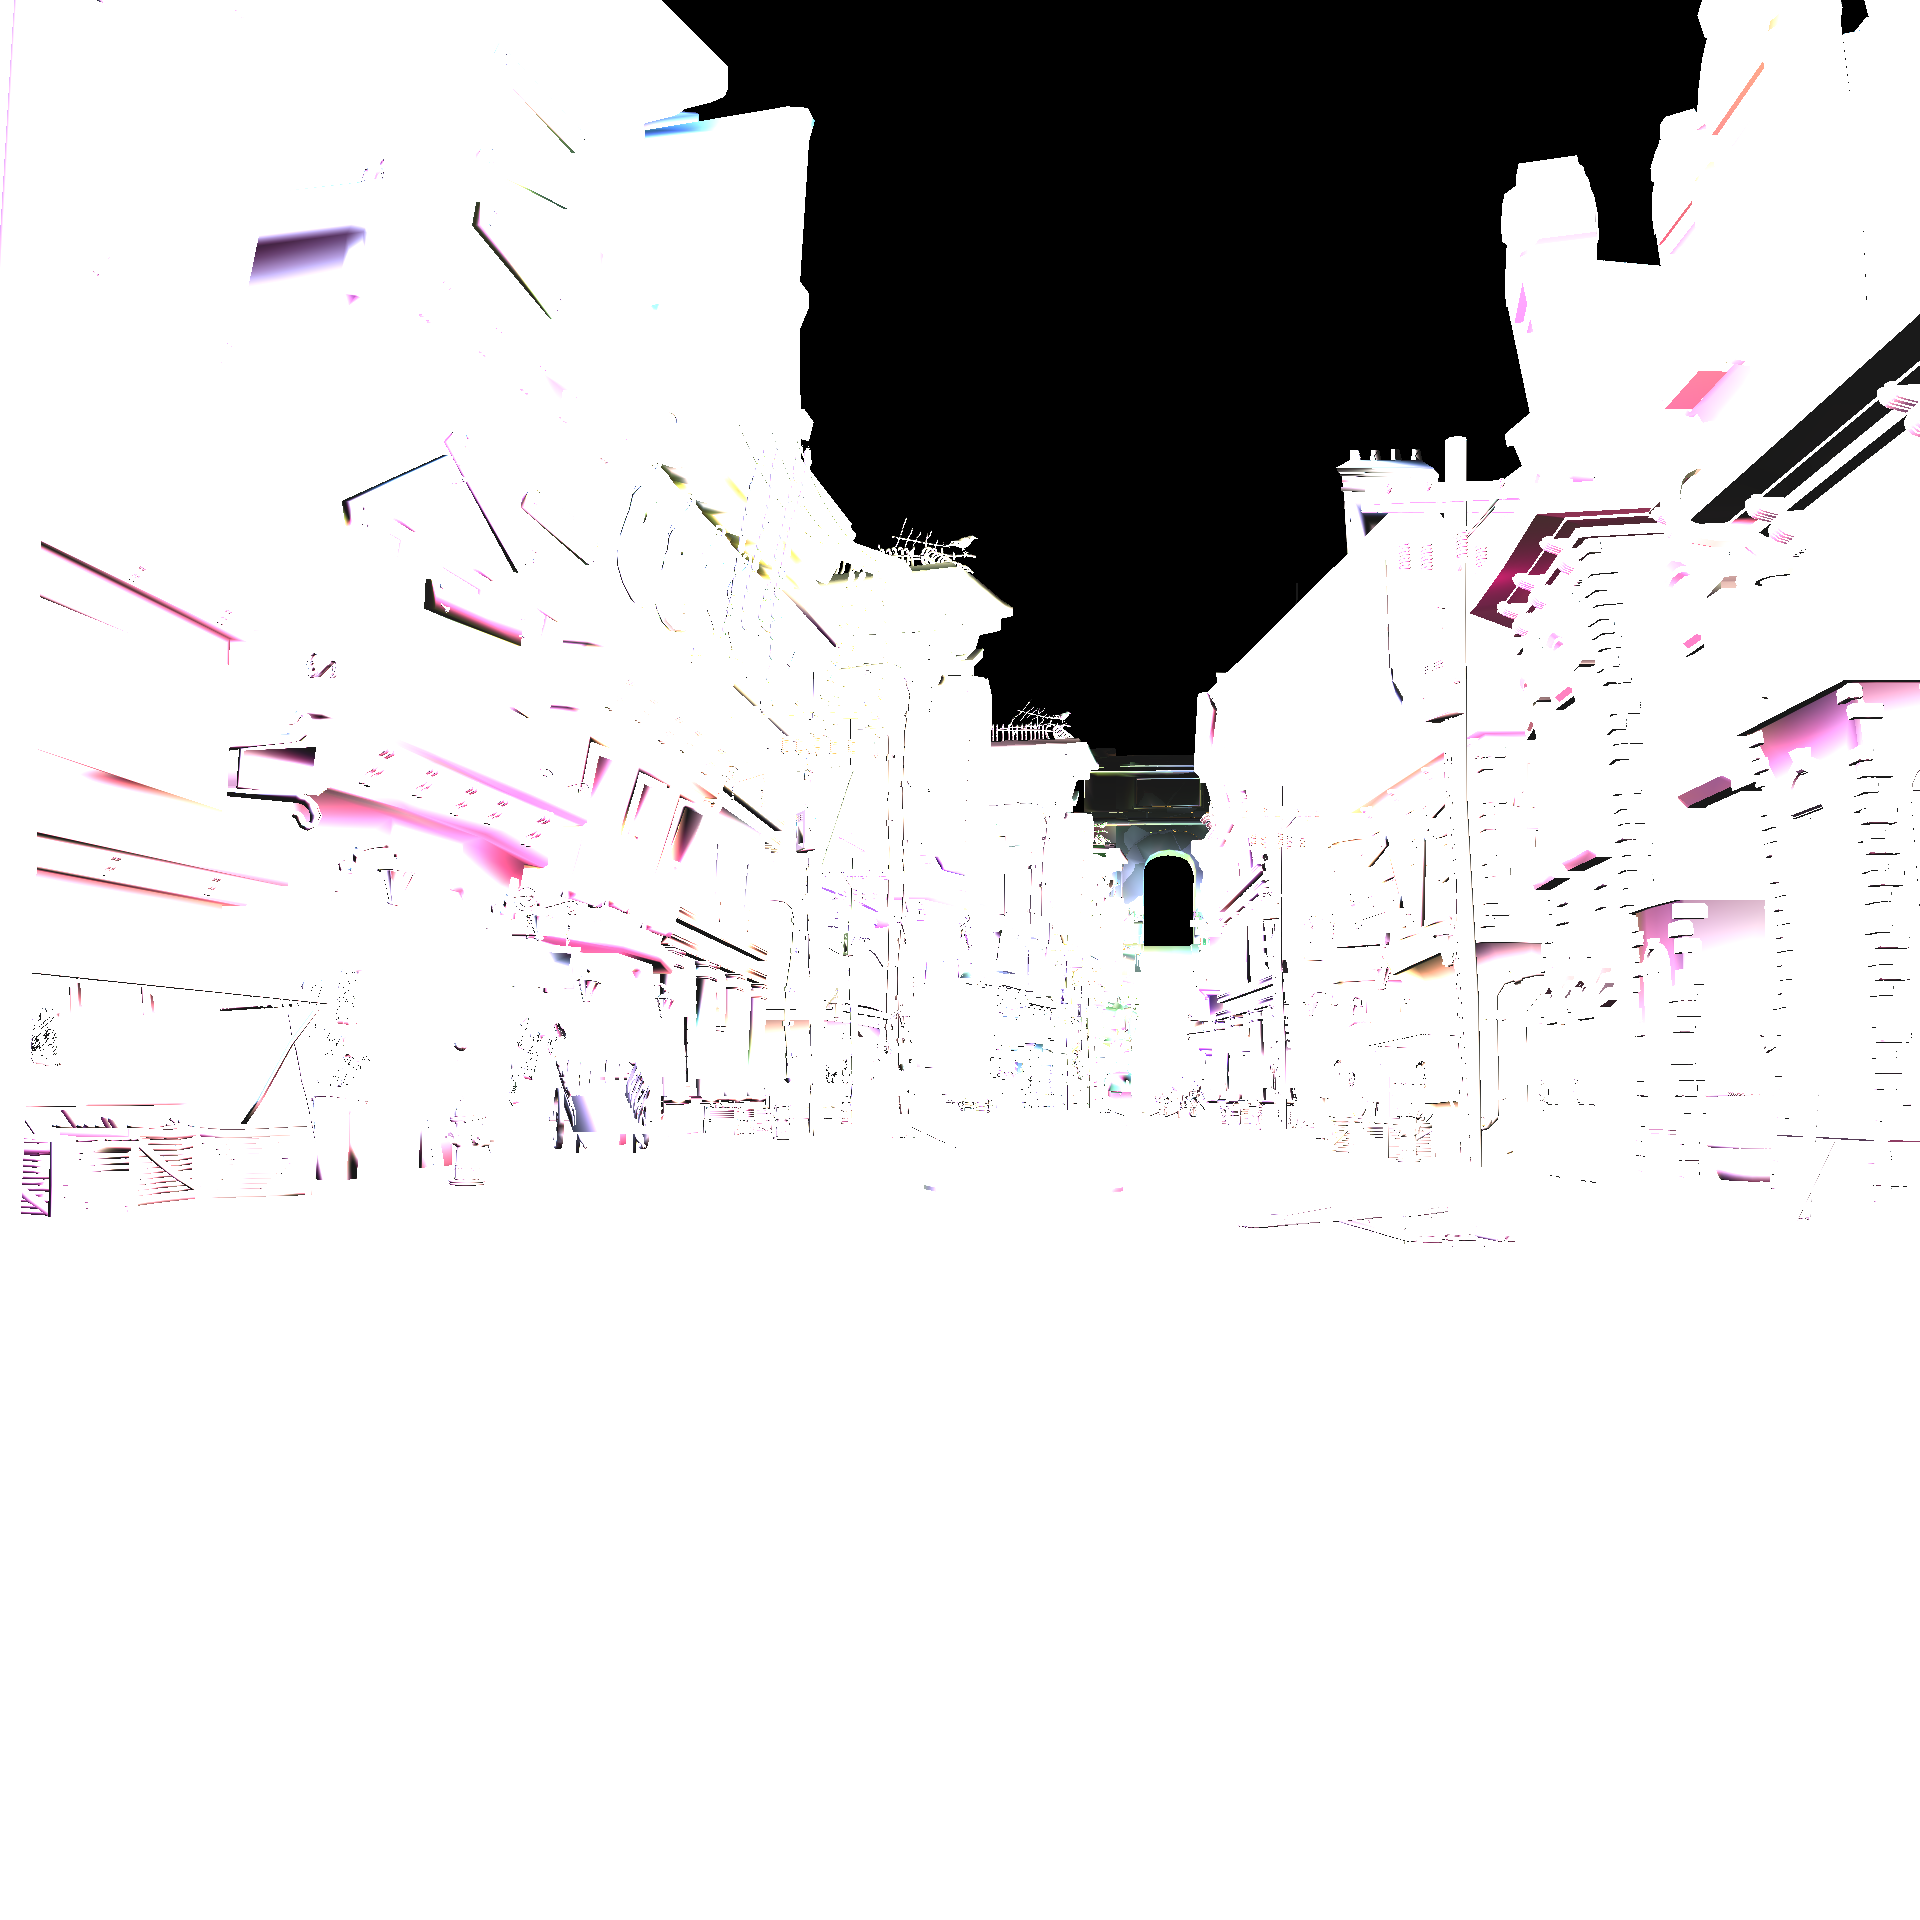
\includegraphics[width=\textwidth]{./img/raw/lc-frame-example/render/pa_frame_126.png}
    \caption{Renderframe $126$.}
    \vspace{2pt}
    \label{fig:ts-test-frames-example:pa:126render}
  \end{subfigure}\quad %
  \begin{subfigure}[b]{0.35\textwidth}
    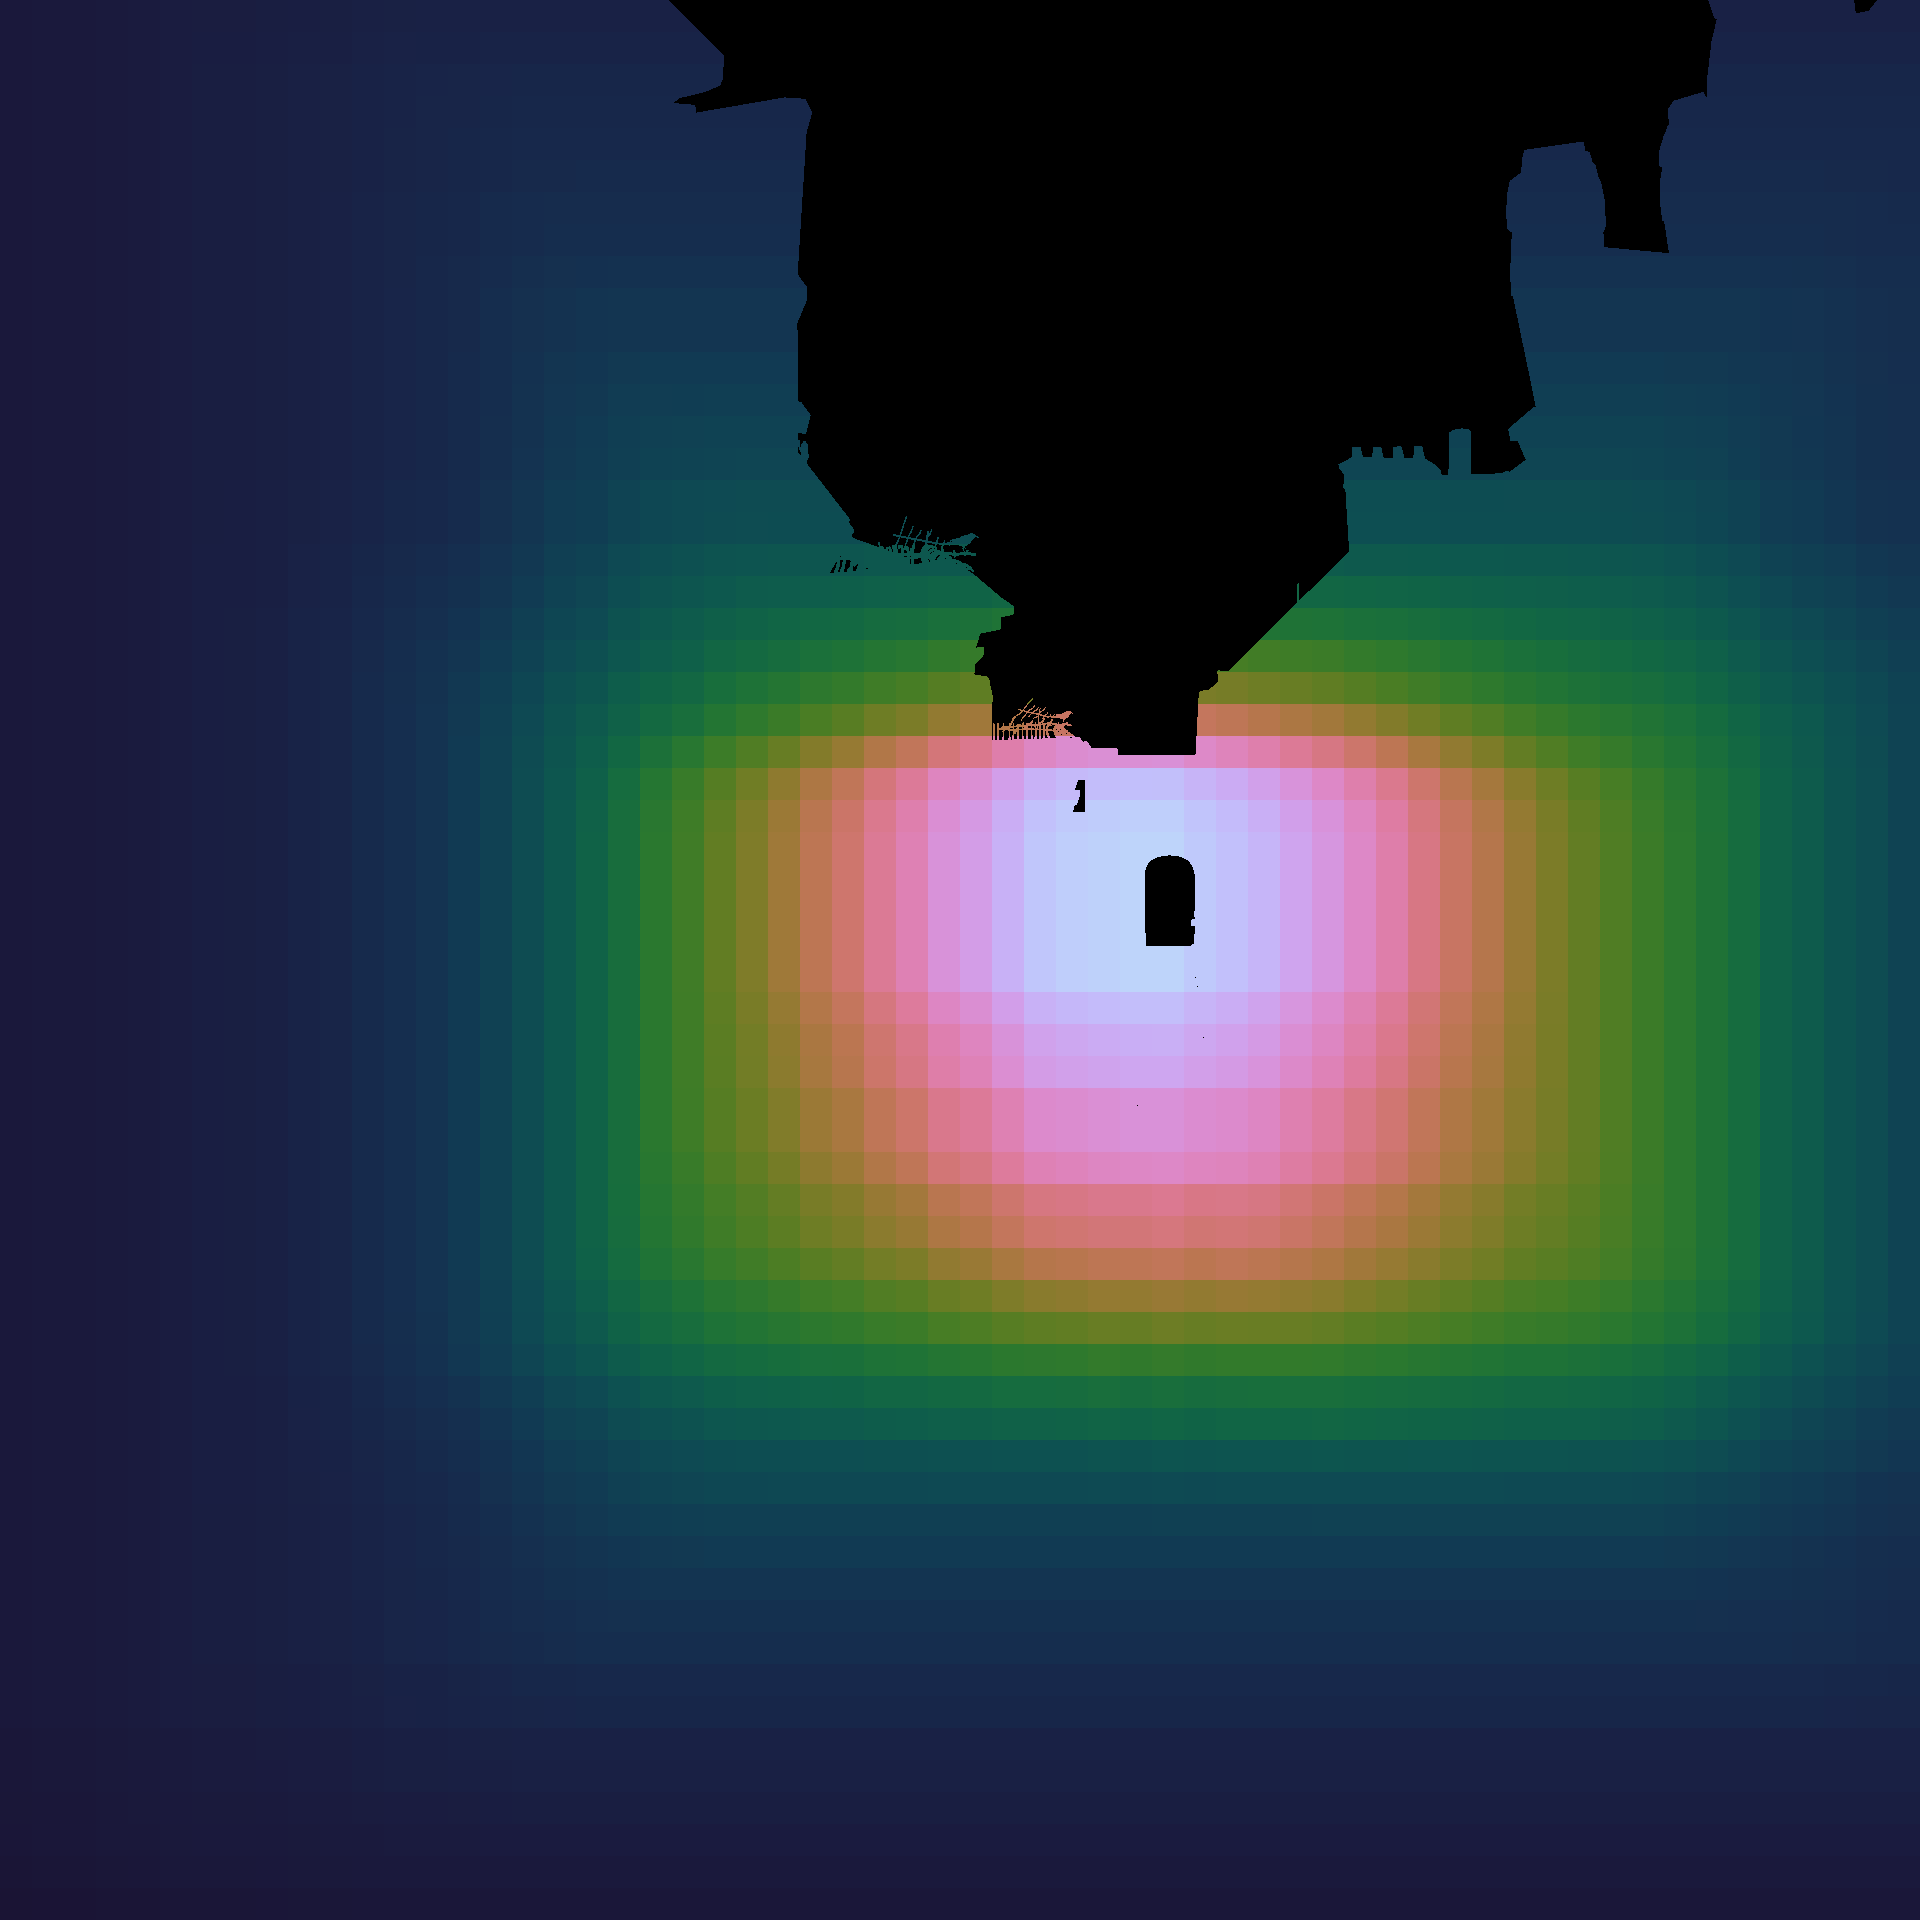
\includegraphics[width=\textwidth]{./img/raw/lc-frame-example/ts/pa_frame_126.png}
    \caption{Lichtberekening frame $126$.}
    \vspace{2pt}
    \label{fig:ts-test-frames-example:pa:126lc}
  \end{subfigure}\\
  \begin{subfigure}[b]{0.35\textwidth}
    
\includegraphics[width=\textwidth]{./img/raw/lc-frame-example/render/zc_frame_417.png}
    \caption{Renderframe $417$.}
    \label{fig:ts-test-frames-example:zc:417render}
  \end{subfigure}\quad %
  \begin{subfigure}[b]{0.35\textwidth}
    
\includegraphics[width=\textwidth]{./img/raw/lc-frame-example/ts/zc_frame_417.png}
    \caption{Lichtberekening frame $417$.}
    \label{fig:fds-test-frames-example:zc417lc}
  \end{subfigure}
  \caption{ Renders en hittekaarten van de verschillende sc\'enes voor Tiled Shading.}
  \label{fig:fds-test-frames-example:zc}
\end{figure}

